\documentclass[11pt]{article}
\usepackage[utf8]{inputenc}
\usepackage[T1]{fontenc}
\usepackage{amsmath}
\usepackage{amssymb} % Needed for \eth
\usepackage{graphicx}
\usepackage{geometry}
\usepackage{tikz}
\usepackage{pgfplots} % For plots
\usepackage{ulem}     % For underline, using normalem to avoid messing with \emph

\geometry{a4paper, margin=1in}
\usetikzlibrary{positioning, arrows.meta, shapes.geometric} % For TikZ diagrams
\pgfplotsset{compat=1.18} % Use a recent PGFPlots version

% Custom commands (optional)
\newcommand{\avg}[1]{\overline{#1}} % Using \bar instead of \overline for simplicity in source
\newcommand{\prob}[1]{P(#1)}
\newcommand{\ProbDens}[1]{\mathcal{P}(#1)} % Using script P for density
\newcommand{\vect}[1]{\vec{#1}}
\newcommand{\dd}[1]{\mathrm{d}#1} % Differential d
\newcommand{\pderiv}[2]{\frac{\partial #1}{\partial #2}}
\newcommand{\deriv}[2]{\frac{\mathrm{d} #1}{\mathrm{d} #2}}
\newcommand{\muState}{\mu\text{-state}} % Microstate
\newcommand{\OmegaE}{\Omega(E)}
\newcommand{\omegaE}{\omega(E)}
\newcommand{\PhiE}{\Phi(E)}
\newcommand{\deltaE}{\delta E}
\newcommand{\ethbar}{\text{\it{đ}}} % \eth symbol for inexact differential
\newcommand{\kb}{k_B} % Boltzmann constant
\newcommand{\tE}{\tilde{E}} % Most probable energy
\newcommand{\tV}{\tilde{V}} % Most probable volume

\title{Physics 415 - Lecture 9: Thermodynamics and Equilibrium}
\date{February 10, 2025}
\author{} % Author not specified

\begin{document}

\maketitle
\thispagestyle{empty}

\section*{Summary}

\begin{itemize}
    \item $\Omega(E) = \#$ accessible states with energy $(E, E+\deltaE)$.
    \item Entropy: $S = \ln \Omega$. (Dimensionless). State function.
    \item Temperature: $\frac{1}{T} = \left( \pderiv{S}{E} \right)_x$. ($T$ in energy units). State function. (Here $x$ represents all fixed external parameters, e.g., $V$).
    \item Interacting systems 1 \& 2 (isolated total): Total entropy $S = S_1 + S_2$ (additive for $N \gg 1$).
    \item Equilibrium corresponds to maximum probability $\implies$ maximum total entropy $S$.
    \item For thermal interaction only ($V_1, V_2$ fixed): Equilibrium condition is $T_1 = T_2$.
    \item For isolated system, spontaneous processes always increase total entropy: $\Delta S \ge 0$.
        \begin{itemize}
            \item Irreversible process: $\Delta S > 0$.
            \item Reversible process: $\Delta S = 0$. (Quasi-static through equilibrium states).
        \end{itemize}
\end{itemize}

\section*{General Interaction Between Macroscopic Bodies}

In general, systems 1 \& 2 interact by exchanging both heat and doing work on each other (e.g., by changing volume).

\begin{center}
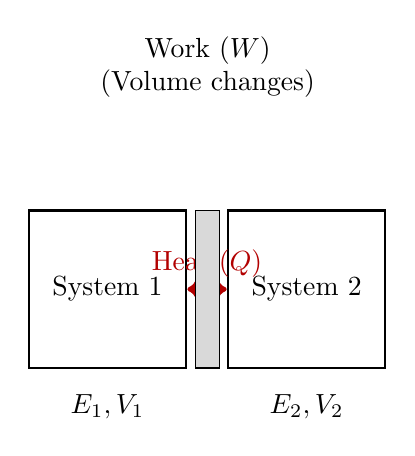
\begin{tikzpicture}
    \node (A) [draw, thick, minimum width=2cm, minimum height=2cm, label=center:System 1] {};
    \node (B) [draw, thick, minimum width=2cm, minimum height=2cm, right=0.5cm of A, label=center:System 2] {};
    % Interface allowing heat exchange & work
    \draw [line width=1.5pt, red!70!black, <->] (A.east) -- (B.west) node [midway, above] {Heat ($Q$)};
    \node (Piston) [draw, fill=gray!30, minimum width=0.3cm, minimum height=2cm, right=0.1cm of A] {}; % Shared piston
    \node at (A.south) [below=0.2cm] {$E_1, V_1$};
    \node at (B.south) [below=0.2cm] {$E_2, V_2$};
    \node [above=1.3cm of Piston, align=center] {Work ($W$) \\ (Volume changes)};
\end{tikzpicture}
\end{center}

Constraints for isolated total system:
\begin{itemize}
    \item $E = E_1 + E_2 = \text{constant}$.
    \item $V = V_1 + V_2 = \text{constant}$. (If total volume is fixed).
\end{itemize}
System 1 state depends on $E_1, V_1$: $\Omega_1 = \Omega_1(E_1, V_1) \implies S_1 = \ln \Omega_1 = S_1(E_1, V_1)$.
System 2 state depends on $E_2, V_2$: $\Omega_2 = \Omega_2(E_2, V_2) \implies S_2 = \ln \Omega_2 = S_2(E_2, V_2)$.
(More generally, $V \to (x_1, x_2, \dots, x_n)$ external parameters). For simplicity, consider single parameter $x=V$. All results generalize easily.

We have seen that, in equilibrium, the distribution for $E_1$ is sharply peaked about $E_1 = \tE_1 = \bar{E}_1$.
Similarly, the distribution of $V_1$ will be sharply peaked about $V_1 = \tV_1 = \bar{V}_1$.
Fluctuations of macroscopic observables about their most probable (=mean) values are entirely negligible. Thus, when referring to macroscopic quantities in equilibrium, we will omit the averaging symbol (e.g., $\bar{E} \to E$, $\bar{p} \to p$, etc.).

\subsection*{Equilibrium Conditions}

Since $S = S(E, V)$, we should make our definition of temperature $T$ more precise:
\[ \frac{1}{T} \equiv \left( \pderiv{S}{E} \right)_V \]
The partial derivative is taken at fixed volume $V$ (and other external parameters $x_\alpha$).
More generally: $\frac{1}{T} = \left( \pderiv{S}{E} \right)_{x_1, x_2, \dots, x_n}$.

Just as with purely thermal interaction, equilibrium is characterized by the maximum of the total entropy $S = S_1 + S_2$. ($S$ is maximized in the most probable state).
We require $dS = dS_1 + dS_2 = 0$ for arbitrary variations $dE_1, dV_1$ (subject to constraints).
$S_1 = S_1(E_1, V_1)$ and $S_2 = S_2(E_2, V_2) = S_2(E-E_1, V-V_1)$.
\[ dS = \left( \pderiv{S_1}{E_1} \right)_{V_1} dE_1 + \left( \pderiv{S_1}{V_1} \right)_{E_1} dV_1 + \left( \pderiv{S_2}{E_2} \right)_{V_2} dE_2 + \left( \pderiv{S_2}{V_2} \right)_{E_2} dV_2 \]
Using the constraints $dE_2 = -dE_1$ and $dV_2 = -dV_1$:
\[ dS = \left[ \left( \pderiv{S_1}{E_1} \right)_{V_1} - \left( \pderiv{S_2}{E_2} \right)_{V_2} \right] dE_1 + \left[ \left( \pderiv{S_1}{V_1} \right)_{E_1} - \left( \pderiv{S_2}{V_2} \right)_{E_2} \right] dV_1 \]
Using $1/T = (\partial S / \partial E)_V$:
\[ dS = \left( \frac{1}{T_1} - \frac{1}{T_2} \right) dE_1 + \left[ \left( \pderiv{S_1}{V_1} \right)_{E_1} - \left( \pderiv{S_2}{V_2} \right)_{E_2} \right] dV_1 \]
For $dS=0$ for arbitrary independent variations $dE_1$ and $dV_1$, the coefficients must be zero:
\begin{enumerate}
    \item $\frac{1}{T_1} - \frac{1}{T_2} = 0 \implies T_1 = T_2$. (Thermal equilibrium condition, as before).
    \item $\left( \pderiv{S_1}{V_1} \right)_{E_1} = \left( \pderiv{S_2}{V_2} \right)_{E_2}$. (New condition related to volume change).
\end{enumerate}

\subsection*{Interpretation of $(\partial S / \partial V)_E$}

What is the physical meaning of $(\partial S / \partial V)_E$?
Consider doing quasi-static, reversible work on a thermally isolated system A.
\begin{itemize}
    \item Reversible $\implies dS = 0$.
    \item Quasi-static work done *by* the system is $\ethbar W = p dV$.
    \item Work done *on* the system is $\ethbar W_{on} = -p dV$.
    \item Thermally isolated $\implies \ethbar Q = 0$.
    \item First Law: $dE = \ethbar Q - \ethbar W = 0 - (p dV) = -p dV$.
\end{itemize}
Now consider the change in entropy $S(E, V)$ during this process. The energy changes by $dE = -p dV$ and volume changes by $dV$. Since $dS=0$:
\[ dS = \left( \pderiv{S}{E} \right)_V dE + \left( \pderiv{S}{V} \right)_E dV = 0 \]
Substitute $dE = -p dV$ and $(\partial S / \partial E)_V = 1/T$:
\[ \left( \frac{1}{T} \right) (-p dV) + \left( \pderiv{S}{V} \right)_E dV = 0 \]
\[ \implies \left[ -\frac{p}{T} + \left( \pderiv{S}{V} \right)_E \right] dV = 0 \]
Since $dV$ can be non-zero, we must have:
\[ \left( \pderiv{S}{V} \right)_E = \frac{p}{T} \]
This gives the physical interpretation of the derivative.

\section*{The Thermodynamic Identity}

We can now write the total differential for entropy $S=S(E,V)$:
\[ dS = \left( \pderiv{S}{E} \right)_V dE + \left( \pderiv{S}{V} \right)_E dV \]
Substituting the definitions we found:
\[ dS = \frac{1}{T} dE + \frac{p}{T} dV \]
Multiplying by $T$: $T dS = dE + p dV$.
Rearranging gives the fundamental thermodynamic identity:
\[ dE = T dS - p dV \qquad (*) \]
This provides a relation between the differentials of macroscopic state functions ($E, S, V$) and state variables ($T, p$) for a system in equilibrium, when undergoing an infinitesimal change from one equilibrium state to another.

\textbf{Example:} Ideal Gas
To illustrate the utility of $(*)$, consider the classical monatomic ideal gas.
Recall from Lecture 4 (using large N approximation): $\Omega(E) \propto V^N E^{3N/2}$.
\[ S = \ln \Omega = N \ln V + \frac{3N}{2} \ln E + \text{constant} \]
(Here $N$ is the number of particles).
\begin{itemize}
    \item Calculate pressure:
    \[ p = T \left( \pderiv{S}{V} \right)_E = T \left( \pderiv{}{V} [N \ln V + \dots] \right)_E = T \left( \frac{N}{V} \right) \]
    \[ \implies pV = NT \]
    This is the ideal gas law! (Note: $T$ is in energy units here. If using Kelvin, $pV = N \kb T$).
    \item Calculate energy relation:
    \[ \frac{1}{T} = \left( \pderiv{S}{E} \right)_V = \left( \pderiv{}{E} [\frac{3N}{2} \ln E + \dots] \right)_V = \frac{3N}{2E} \]
    \[ \implies E = \frac{3}{2} NT \]
    This is the (mean) energy of a classical monatomic ideal gas.
\end{itemize}
The relation $pV=NT$ (or similar relations for other systems) is an example of an "equation of state", which is a relation connecting quantities characterizing a macroscopic equilibrium state.

\section*{Connection to Heat}

There is another important application of the result $dE = T dS - p dV \quad (*)$.
Recall the First Law: The change in (mean) energy $dE$ is due to infinitesimal heat absorbed $\ethbar Q$ and work done *by* the system $\ethbar W$:
\[ dE = \ethbar Q - \ethbar W \]
Consider the special case of a quasi-static process. We have shown that for such processes, the work done by the system involving volume change is $\ethbar W = p dV$.
\[ \implies dE = \ethbar Q - p dV \quad (\text{for quasi-static process}) \]
Comparing this to the thermodynamic identity $(*)$:
\[ T dS - p dV = \ethbar Q - p dV \]
\[ \implies T dS = \ethbar Q \]
or
\[ dS = \frac{\ethbar Q}{T} \qquad (**) \]
This provides a crucial relation between the change in entropy $dS$ (an exact differential) and the heat absorbed $\ethbar Q$ (an inexact differential) \underline{in a quasi-static process}.

\textbf{Special Case:} Quasi-static process in a thermally isolated system ($\ethbar Q = 0$).
From $(**)$, we have $dS = 0$, so $S = \text{constant}$.
If quasi-static work is done on (or by) a thermally isolated system, the entropy does not change. Such a process is reversible ($dS_{tot}=0$).

Equation $(**)$ is also notable because it relates the inexact differential $\ethbar Q$ to the exact differential $dS$ via the integrating factor $1/T$.
Since $S$ is a function only of the macrostate (e.g., $S=S(E,V)$), the change in entropy between any initial equilibrium state $i$ and final equilibrium state $f$ is:
\[ \Delta S = S_f - S_i = \int_i^f dS = \int_i^f \frac{\ethbar Q}{T} \]
The integral $\int \ethbar Q / T$ must be calculated along \underline{any quasi-static (reversible) path} connecting states $i$ and $f$. Because $S$ is a state function, the value of this integral is independent of the reversible path chosen.

\begin{center}
\begin{tikzpicture}
\begin{axis}[
    axis lines=middle, xlabel=$V$, ylabel=$p$,
    xmin=0, xmax=5, ymin=0, ymax=4,
    xtick=\empty, ytick=\empty,
    width=7cm, height=5cm
]
\coordinate (i) at (axis cs:1, 3);
\coordinate (f) at (axis cs:4, 1);
\node at (i) [circle, fill=black, inner sep=1.5pt, label=above left:i] {};
\node at (f) [circle, fill=black, inner sep=1.5pt, label=below right:f] {};

% Path 1 (reversible)
\draw [thick, blue, ->] (i) .. controls (2,2.5) and (3,1.5) .. (f) node[midway, above right] {(1)};
% Path 2 (reversible)
\draw [thick, red, dashed, ->] (i) -- (f) node[midway, below left] {(2)};

\node [align=center] at (axis cs:2.5, 0.5) {$\int_{(1)} \frac{\ethbar Q}{T} = \int_{(2)} \frac{\ethbar Q}{T} = S_f - S_i$};
\end{axis}
\end{tikzpicture}
\end{center}

\section*{Equilibrium Conditions Revisited}

Finally, return to the initial problem of equilibrium between systems 1 \& 2 allowing both energy and volume exchange.
The equilibrium conditions derived from maximizing $S=S_1+S_2$ ($dS=0$) were:
\begin{enumerate}
    \item $T_1 = T_2$ (Thermal equilibrium).
    \item $\left( \pderiv{S_1}{V_1} \right)_{E_1} = \left( \pderiv{S_2}{V_2} \right)_{E_2}$.
\end{enumerate}
Using the relation $(\partial S / \partial V)_E = p/T$, the second condition becomes:
\[ \frac{p_1}{T_1} = \frac{p_2}{T_2} \]
Since we already have $T_1 = T_2$ from the first condition, this implies:
\[ p_1 = p_2 \]
This is the condition for "mechanical equilibrium".

Thus, in full equilibrium, systems 1 \& 2 have equal temperatures ($T_1=T_2$) and the pressure is balanced ($p_1=p_2$).

(Note: Mechanical equilibrium (equality of pressures) is often reached much more rapidly than thermal equilibrium (equality of temperatures)).

\end{document}